\documentclass[conference]{IEEEtran}

\usepackage{cite}
\usepackage{amsfonts,amsmath,amssymb,amsthm,booktabs,color,enumitem,graphicx}
\usepackage{float}


% correct bad hyphenation here
\hyphenation{op-tical net-works semi-conduc-tor}


\begin{document}

\title{Pipeline for Continuous Deployment and Continuous Experimentation}

\author{\IEEEauthorblockN{Olli Rissanen}
\IEEEauthorblockA{Department of Computer Science\\
University of Helsinki\\
Helsinki, Finland\\
Email: olli.rissanen@helsinki.fi}}

% make the title area
\maketitle

\begin{abstract}
An important principle in lean software development is to deliver features as fast as possible, in order to reduce the length of feedback cycles and to readily address customer's present needs. A way to shorten the delivery cycles is to adopt continuous deployment. Continuous deployment is a design practice in which software delivery process is automated and software is constantly deployed to customer environment. However, adopting continuous deployment doesn't necessarily mean that more value is created for the customer, and customer feedback might not be properly collected. While continuous deployment attempts to deliver an idea to users as fast as possible, continuous experimentation instead attempts to validate that it is, in fact, a good idea. In a state of continuous experimentation, the entire R\&D process is guided by controlled experiments and feedback. In its core continuous experimentation consists of a design-execute-analyse loop, where hypotheses are selected based on business goals and strategies, experiments are executed with partial implementations and data collection tools and finally the results are analyzed to validate the hypothesis. In this paper we're conducting a literature review on the pipelines for continuous deployment and continuous experimentation. The main research questions are how to create a pipeline for continuous experimentation, which components are required for such a pipeline and whether this pipeline should be integrated to the deployment pipeline. 
\end{abstract}
% IEEEtran.cls defaults to using nonbold math in the Abstract.
% This preserves the distinction between vectors and scalars. However,
% if the conference you are submitting to favors bold math in the abstract,
% then you can use LaTeX's standard command \boldmath at the very start
% of the abstract to achieve this. Many IEEE journals/conferences frown on
% math in the abstract anyway.
\begin{IEEEkeywords}
Continuous deployment, Continuous experimentation, Deployment pipeline
\end{IEEEkeywords}

% For peer review papers, you can put extra information on the cover
% page as needed:
% \ifCLASSOPTIONpeerreview
% \begin{center} \bfseries EDICS Category: 3-BBND \end{center}
% \fi
%
% For peerreview papers, this IEEEtran command inserts a page break and


% creates the second title. It will be ignored for other modes.
\IEEEpeerreviewmaketitle

%Perusteet

%Kiinnostava
%Innostava
%Tehtävissä

%Määrittele
% Tutkimusongelma, siis mitä haluat ymmärtää tai selvittää
% Tavoitteet
% Menetelmät
% Rajaus

%Mahdollisia toteutustapoja
% Vertaile kahta tai useampaa lähestymistapaa
% Etsi empiiristä todistusaineistoa jonkin väitteen puolesta tai sitä vastaan
% Kuvaa tapausyrityksen tilanne ja vertaile kirjallisuuteen
%

%Haasteet

%In fact, one sign of a good application architecture is that it allows the application
%to be run without much trouble on a development machine.

\section{Introduction} %why is this problem interesting?
Lean software development is a translation of both lean manufacturing and lean IT principles to software development domain \cite{poppendieck2003lean}. It consists of seven principles, such as "Eliminate waste" and "Deliver as fast as possible". Shortening the delivery cycle both shortens the time it takes to receive customer feedback for a release, and assures that customer's present needs can be addresses readily. Automating the delivery process further reduces human error, documents required for the build and increases confidence that the build works \cite{cdbook}.

A way to shorten the delivery cycles and to automate the delivery process is continuous deployment. It is an extension to continuous integration, where the delivery process is often entirely automated, and software functionality is deployed frequently to customer environment. While continuous integration defines a process where the work is automatically built, tested and frequently integrated to mainline \cite{fowler2006continuous}, often multiple times a day, continuous deployment adds automated acceptance testing and deployment.. %Explain pipeline here

An important part of continuous deployment is the deployment pipeline, which is an automated implementation of an application's build, deploy, test and release process \cite{cdbook}. A deployment pipeline can be loosely defined as a consecutively executed set of validations that a software has to pass such before it can be released. Common components of the deployment pipeline are a version control system and an automated test suite.

In an agile process software release is done in periodic intervals \cite{cockburn2002agile}. Compared to waterfall model it introduces multiple releases throughout the development. Continuous deployment, on the other hand, attemps to keep the software ready for release at all times during development process \cite{cdbook}. Instead of stopping the development process and creating a build as in an agile process, the software is continuously deployed to customer environment. This doesn't mean that the development cycles in continuous deployment are shorter, but that the development is done in a way that makes the software always ready for release.

It should also be made clear that continuous delivery differs from continous deployment. Refer to Fig. \ref{fig1} for a visual representation of differences in continuous integration, delivery and deployment. Both include automated deployment to a staging environment. Continuous deployment includes deployment to a production environment, while in continuous delivery the deployment to a production environment is done manually. The purpose of continuous delivery is to prove that every build is proven deployable \cite{cdbook}. While it necessarily doesn't mean that teams release often, keeping the software in a state where a release can be made instantly is often seen beneficial.

\begin{figure}[!t]
	\centering
	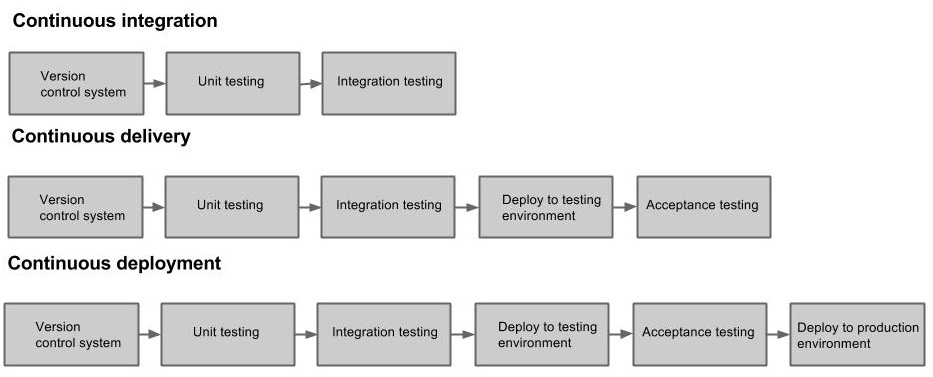
\includegraphics[width=3.5in]{rtvd.jpg}
	\caption{Continuous integration, delivery and deployment}
	\label{fig1}
\end{figure}

Adopting a continuous deployment process doesn't necessarily mean that more value is delivered to a customer. Avinash Kaushik states in his Experimentation and Testing primer \cite{kaushik} that "80\% of the time you/we are wrong about what a customer wants". Mike Moran also found similar results in his book Do It Wrong Quickly, stating that Netflix considers 90\% of what they try to be wrong. A way to tackle this issue is to adopt a process of continuous experimentation, where the entire R\&D system responds and acts based on instant customer feedback, and where actual deployment of software functionality is seen as a way of experimenting and testing what the customer needs \cite{olsson2012climbing}.
 
Continuous deployment attempts to deliver an idea to users as fast as possible. Continuous experimentation instead attempts to validate that it is, in fact, a good idea. In continuous experimentation the organisation runs controlled experiments to guide the R\&D process. The development cycle in continuous experimentation resembles the build-measure-learn cycle of lean startup \cite{ries2011lean}. The process in continuos experimentation is to first form a hypothesis based on a business goals and customer "pains" \cite{bosch2012building}. After the hypothesis has been formed, quantitative metrics to measure the hypothesis must be decided. After this a minimum viable product can be developed and deployed, while collecting the required data. Finally, the data is analyzed to attempt to validate the hypothesis.

As the experiments are run in a regular fashion, it should be considered to attempt to integrate experiments to the deployment pipeline. This requires changing the development process in such fashion that functionality is developed based on validated hypotheses. The components required to support continuous experimentation include tools to assign users to treatment and control groups, tools for data logging and storing, and analytics tool for conducting statistical analyses.

In this paper we investigate the pipelines for continuous deployment and continuous experimentation, and the main research questions are how to create a pipeline for continuous experimentation, which components are required for such a pipeline and whether this pipeline should be integrated to the deployment pipeline. 

This paper is organized as follows. Chapter II explains the research approach and the selection of cited papers. Chapter III presents the results from literature review, exploring the deployment pipeline, experimentation in software engineering and components required for a continuous experimentation pipeline. Chapter IV then applies these findings to create a draft of a pipeline for continuous experimentation. Future research is introduced briefly in Chapter V. Finally, Chapter VI concludes the paper with key points.

\section{Methods} %how did I find the papers? %TODO: UPDATE THIS %Kerro tarkemmin kuin vaan mitä hakuja tehtiin

Articles were found by tracking the citations from the article Climbing the "Stairway to Heaven" -- A Multiple-Case Study Exploring Barriers in the Transition from Agile Development towards Continuous Deployment of Software \cite{olsson2012climbing}, and by reading through the publishings of Experimentation Platform \cite{ep}. Articles on continuous delivery and deployment are easily available, but continuous experimentation is still a relatively new concept. Also the term continuous experimentation is often replaced with innovation experiment system, for example.

What resulted from the citations of "Stairway to Heaven" article was mostly theoretical research on experiments, lean methodologies, continuous delivery and data analysis. Applied studies on continuous experimentation were found from the Microsoft Experimentation Platform, but they mostly consisted of A/B testing on web sites. Practical implementations of continuous experimentations were not found in the scientific papers apart from a few short cases \cite{bosch2012building}. However, enough information on restrictions and components were found such that a rough draft can be made.

The research supporting continuous experimentation, such as statistical analysis, mapping backlogs to roadmaps and using experiments to validate hypotheses were found in vast amounts. Practical implementations of continuous delivery and deployment are also readily available.

\section{Results} %Pure analysis on the papers

A deployment pipeline for continuous deployment consists of the phases a build has to pass in order for it to be deployed. A pipeline for continuous experimentation, on the other hand, consists of the steps required to design, execute and analyse an experiment. The cycle of continuous experimentation resembles the build-measure-learn cycle of lean startup \cite{ries2011lean}. In continuous experimentation, the main process is to form a new hypothesis, decide on quantitative metrics, deploy new functionality, measure the previously decided metrics and subsequently use the collected data to drive development \cite{bosch2012building}. In this chapter we first introduce the pipeline for continous deployment, then investigate experimentation in software engineering and components required to implement a pipeline for continuous experimentation. In the next chapter, we apply these findings to create a draft of a pipeline for continuous experimentation.

\subsection{Pipeline for continuous deployment \footnote{This section poses similarities to the author's article Importance of Software Architecture in Continuous Deployment. For more information on the subject, refer to the aforementioned article.}}	

The primary purpose of continuous deployment is to improve the process of software delivary. This is done by automating the whole deployment process, since unless deployments are automated, errors will occur every time they're performed \cite{cdbook}. The components of a deployment pipeline typically are a version control system and an automated test suite consisting of unit tests, integration tests and acceptance tests. 

Humble and Farley define the deployment pipeline as a set of stages, which cover the path from a committed change to a build \cite{cdbook}. Refer to Fig. \ref{fig2} for a graphical representation of a basic deployment pipeline. The commit stage compiles the build and runs code analysis, while acceptance stage runs an automated test suite that asserts the build works at both functional and nonfunctional level. From there on, builds to different environments can be deployed either automatically or by a push of a button.

Humble et al. define four principles that should be followed when attempting to automate the deployment process \cite{humble2006deployment}. The first principle states that "Each build stage should deliver working software". As software often consists of different modules with dependencies to other modules, a change to a module could trigger builds of the related modules as well. Humble et al. argue that it is better to keep builds separate so that each discrete module could be built individually. The reason is that triggering other builds can be inefficient, and information can be lost in the process. The information loss is due to the fact that connection between the initial build and later builds is lost, or at least causes a lot of unnecessary work spent in tracing the triggering build. 

The second principle states that "Deploy the same artifacts in every environment". This creates a constraint that the configuration files must be kept separate, as different environments often have different configurations. Humble et al. state that a common anti-pattern is to aim for 'ultimate configurability', and instead the simplest configuration system that handles the cases should be implemented.
\begin{figure}[H]
	\centering
	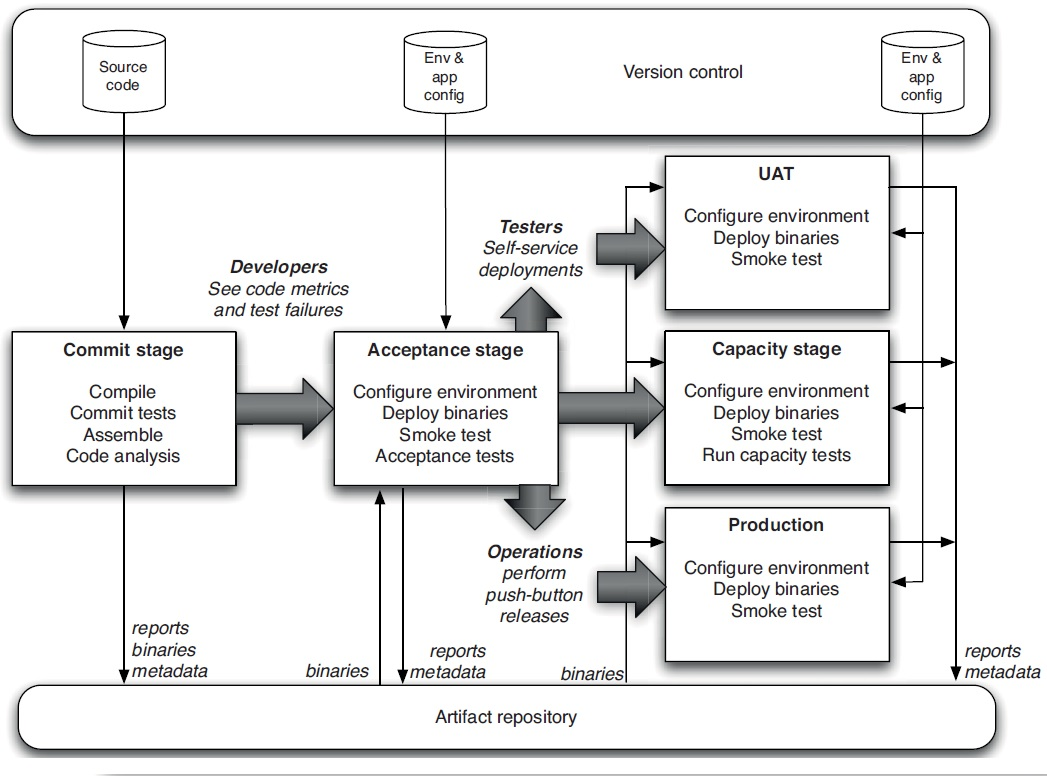
\includegraphics[width=3.5in]{pipeline.jpg}
	\caption{A basic deployment pipeline \cite{cdbook}.}
	\label{fig2}
\end{figure}
Another principle, which is the main element of continuous deployment, is to "Automate testing and deployment". Humble et al. argue that the application testing should be separated out, such that stages are formed out of different types of tests. This means that the process can be aborted if a single stage fails. They also state that all states of deployment should be automated, including deploying binaries, configuring message queues, loading databases and related deployment tasks. Humble et al. mention that it might be necessary to split the application environment into $slices$, where each slice contains a single instance of the application with predetermined set of resources, such as ports and directories. $Slices$ make it possible to replicate an application multiple times in an environment, to keep distinct version running simultaniously. Finally, the environment can be smoke tested to test the environments capabilities and status.

The last principle states "Evolve your production line along with the application it assembles". Humble et al. state that attempting to build a full production line before writing any code doesn't deliver any value, so the production line should be built and modified as the application evolves. 

A picture of the typical development process in continuous deployment is shown in Fig. \ref{fig3}. After the team pushes a change to the version control system, the project is automatically built and tests are triggered stage by stage. If a test stage fails, feedback is given and the deployment process effectively cancelled. In a continuous delivery process, the last stages are approved and activated manually, but in a continuous deployment process the last stages are triggered automatically as well.

\begin{figure}[!t]
	\centering
	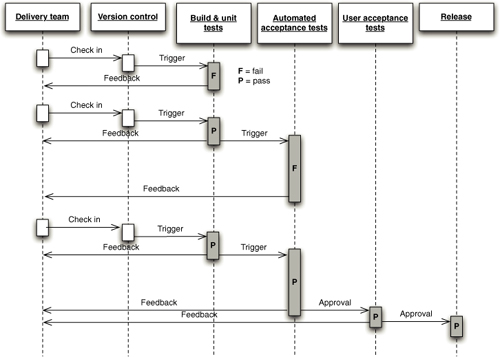
\includegraphics[width=3.5in]{developmentprocess.jpg}
	\caption{Components of the development process \cite{cdbook}.}
	\label{fig3}
\end{figure}

\subsection{Experimentation}

An experiment is essentially a procedure to confirm the validity of a hypothesis. In software engineering context, experiments attempt to answer questions such as which features are necessary for a product to succeed, what should be done next and which customer opinions should be listened to. According to Jan Bosch, "The faster the organization learns about the customer and the real world operation of the system, the more value it will provide" \cite{bosch2012building}. Most organizations have many ideas, but the return-on-investment for many may be unclear and the evaluation itself may be expensive \cite{kohavi2007practical}. I

In Lean startup methodology \cite{ries2011lean} experiments consist of Build-Measure-Learn cycles, and are tightly connected to visions and the business strategy. The purpose of a Build-Measure-Learn cycle is to turn ideas into products, measure how customers respond to the product and then to either pivot or persevere the chosen strategy. The cycle starts with forming a hypothesis and building a minimum viable product (MVP) with tools for data collection. Once the MVP has been created, the data is analyzed and measured in order to validate the hypothesis. To persevere with a chosen strategy means that the experiment proved the hypothesis correct, and the full product or feature can is implemented. However, if the experiment proved the hypothesis wrong, the strategy is changed based on the implications of a false hypothesis.

Jan Bosch has widely studied continuous experimentation, or innovation experiment systems, as a basis for development. The primary issue he found is that "experimentation in online software is often limited to optimizing narrow aspects of the front-end of the website through A/B testing and inconnected, software-intensive systems experimentation, if applied at all, is ad-hoc and not systematically applied" \cite{bosch2012building}. The author realized that for different development stages, different techniques to implement experiments and collect customer feedback exist. Bosch also introduces a case study in which a company, Intuit, adopted continuous experimentation and has increased both the performance of the product and customer satisfaction.

Fig. \ref{fig4} introduces different stages and scopes for experimentation. For example A/B testing is not always beneficial, and the continuous experimentation process must consider other forms of experiments as well. For each stage and scope combination, an example technique to collect product performance data is shown. As startups often start new products and older companies instead develop new features, experiments must be applied in the correct context. Bosch states that for a new product deployment, putting a minimal viable product as rapidly as possible in the hands of customers is essential \cite{bosch2012building}. After the customers can use the product, it is often not yet monetizable but is still of value to the customer. Finally, the product is commercially deployed and collecting feedback is required to direct R\&D investments to most valuable features.
\begin{figure}[H]
	\centering
	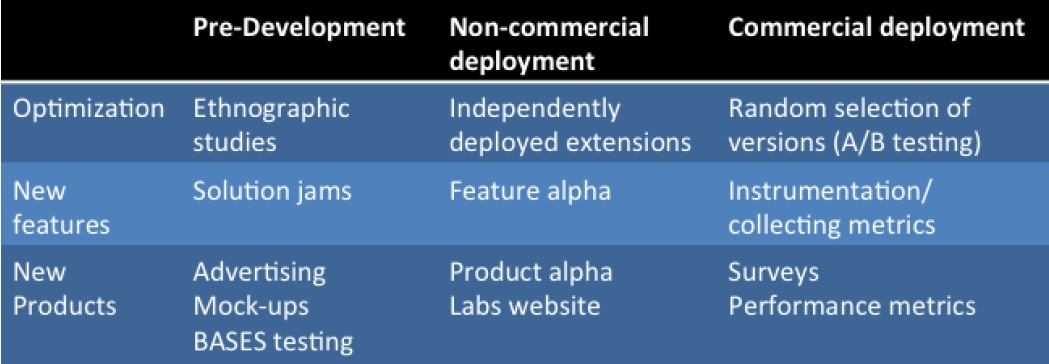
\includegraphics[width=3.5in]{bosch.jpg}
	\caption{Scopes for experimentation\cite{bosch2012building}.}
	\label{fig4}
\end{figure}
Crook et al. investigated the common pitfalls encountered when running controlled experiments on the web \cite{crook2009seven}, which are listed in Table II. The Overall Evaluation Criteria (OEC) used in the first pitfall is a quantitative measure of the experiment's objective. In experimental design, Control is a term used for the existing feature or a process, while a Treatment is used to describe a modified feature or a process. As a motivator for the first pitfall, Crook et al. introduce an experiment where the OEC was set to the time spent on a page which contains articles. The OEC increased in the experiment implementation, satisfying the objective. However, it was soon realized that the longer time spent on a page might have been caused by confusion of the users, as a newly introduced widget was used less often than a previous version of it. 

Aside from picking a correct OEC, common pitfalls deal with the correct use of statistical analysis, robot users such as search engine crawlers, and the importance of audits and control.
\begin{center}
\begin{table}[htb]
    \begin{tabular}{ | p{1cm} | p{6cm} |}
    \hline
	Pitfall 1 & Picking an OEC for which it is easy to beat the control by doing something clearly “wrong” from a business perspective \\ \hline
	Pitfall 2 & Incorrectly computing confidence intervals for percent change and for OECs that involve a nonlinear combination of metrics \\ \hline
	Pitfall 3 & Using standard statistical formulas for computations of variance and power \\ \hline
	Pitfall 4 & Combining metrics over periods where the proportions assigned to Control and Treatment vary, or over subpopulations sampled at different rates \\ \hline
	Pitfall 5 & Neglecting to filter robots \\ \hline
	Pitfall 6 & Failing to validate each step of the analysis pipeline and the OEC components \\ \hline
	Pitfall 7 & Forgetting to control for all differences, and assuming that humans can keep the variants in sync \\ \hline
    \end{tabular}
    \caption{Pitfalls to avoid when running controlled experiments on the web \cite{crook2009seven}.}
    \end{table}
\end{center}
%Experimentation doesn't necessarily require development of software.

\subsection{Components in continous experimentation}

Kohavi et al. investigate the practical implementations of controlled experiments on the web \cite{kohavi2007practical}, and state that the implementation of an experiment involves two components. The first component is a randomization algorithm, which is used to map users to different variants of the product in question. The second component is an assignment method which, based on the output of the randomization algorithm, determines the contents that each user are shown. The observations then need to be collected, aggregated and analyzed to validate a hypothesis. Kohavi et al. also state that most existing data collection systems are not designed for the statistical analyses that are required to correctly analyze the results of a controlled experiment.

The components introduced by Kohavi et al. are aimed primarily for A/B testing on websites. Three ways to implement the assignment methods are shown. The first one is traffic splitting, which directs users to different fleet of servers. An alternative methods is server-side selection, in which API calls invoke the randomization algorithm and branch the logic based on the return value. Last alternative is a client-side selection, in which the front-end system dynamically modifies the page to change the contents. Kohavi et al. state that the client-side selection are easier to implement, but it severely limits the features that may be subject to experimentation. Experiments on back-end are nearly impossible to implement in such manner.

To collect, aggregate and analyze the observations, raw data has to be recorded. According to Kohavi et al., some raw data could be for example page views, clicks, revenue, render time and customer-feedback selections. The data should also be annotated to an identifier, such that conclusions can be made from it. Kohavi et al. present three different ways for collecting raw data. The first solution is to simply use an existing data collection tool, such as Webmetrics. However, most data collection systems aren't designed for statistical analyses, and the data might have to be manually extracted to an analysis environment. A different approach is local data collection, in which a website records data in a local database or log files. The problem with local data collection is that each additional source of data, such as the back-end, increases the complexity of the data recording infrastructure. The last model is a service-based collection, in which service calls to a logging service are placed in multiple places. This centralizes all observation data, and makes it easy to combine both back-end and front-end logging.  

To analyze the raw data, it must first be converted into metrics which can then be compared between the variants in a given experiment. An arbitrary amount of statistical tests can then be run on the data with analytics tools in order to determine statistical significance. 

\section{Discussion} %Own speculation

A system with continuous experimentation must be able to release minimum viable products with integrated data collection instruments in a rapid manner. The process of continuous experimentation requires tools for designing, executing and analyzing experiments. Designing experiments should be tied to strategic goals, and high emphasis should be directed towards deciding the correct quantitative measurements. Executing experiments requires a set of tools used for collecting the data for previously selected metrics. In case of A/B tests logic that divides users to treatment and control is required. For analyzing the data, analytical tools and database to store both the raw data and results are required. Finally, a database for storing information on experiments, such as the raw data, is required.

The deployment pipeline introduced in Chaper II makes it possible to effectively deploy new features to the customer environment. Based on the purpose of the deployment pipeline - to automate the deployment process - it would seem unnecessary to attempt to add more components to the deployment pipeline, and instead consider it as a prequisite that enables effective continuous experimentation. Due to the ability to near instantly deploy new features, minimum viable products can be both deployed and ejected quickly. The continuous experimentation pipeline should, however, be tightly linked to the deployment pipeline, such that arbitrary experiments can be deployed at will. Emphasis should also be paid to implementing the back-end system in such manner that experimentations and minimum viable products can be quickly, possibly even automatically, created. 

By building the logging component as a service that can be integrated to an existing application in the sense suggested by Kohavi et al. \cite{kohavi2007practical}, the data collection can quickly and efficiently be added to products or features. 

The implementation of continuous experimentation is highly dependant on the company and product in question. In a SaaS product, where users access the providers services, adding data collection instruments and tracking user actions is relatively simple. This also applies to websites. However, in embedded systems or unfrequently deployed larger applications the approach is different, and multiple environments might be needed for testing. In some cases, following the process of continuous experimentation might not even be viable at all. Another issue lies at the user base. Larger the user base is, the more comprehensive and reliable is the statistical data. 

\begin{figure}[H]
	\centering
	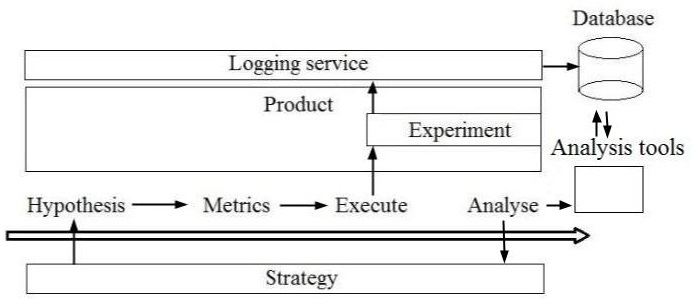
\includegraphics[width=3.5in]{cepl.jpg}
	\caption{Pipeline for continuous experimentation.}
	\label{fig5}
\end{figure}

Compared to the build-measure-learn cycle of Lean startup \cite{ries2011lean}, the cycle in continuous experimentation can be defined as hypothesis-metric-experiment-analyse. Refer to Fig. \ref{fig5} for a visual representation. The pipeline therefore begins with choosing a hypothesis and metrics required to validate the hypothesis. The execute phase includes implementing the minimum viable product, attaching it to the logging component and deploying it to the desired environment. The data is then analyzed and the hypothesis validated. Finally, the product can be updated or removed based on the results of the data, and the business strategy changed accordingly. Based on the infrastructure of the company in question, different stakeholders can be responsible for each stage. Fagerholm et al. have also created a draft of a pipeline for continuous experimentation, along with the general continuous experimentation infrastructure model \cite{fagerholm2014building}.

%Based on the studies by Kohavi et al., in 
%The quantitative measure must be correct (pitfall)
%What kind of elements need to be added to the deployment pipeline based on these papers?
%The pipeline for continuous deployment
%The pipeline for continuous experimentation
%Based on the features required by .., a set of restrictions can be ..

%Restrictions
%\#1 Running an experiment should be optional, and deploying without experimenting must be made possible

\section{Future research} %Self-explanatory
Olsson et al. are planning to research the transition from continuous deployment to an experiment system in their future research. The research is continuing from their earlier research on transitioning from traditional methodologies to agile methodologies, and further to continuous deployment. \cite{olsson2012climbing}

Jan Bosch intends to apply the Innovation Experiment Systems to practice, similar to the authors previous case study on an industrial case, Intuit \cite{bosch2012building}.

The author of this paper is studying the transition from continuous deployment to continuous experimentation in an industrial case study.
\section{Conclusion} %Short wrap-up. Contains the key points

The deployment pipeline is an automated implementation of an application's build, deploy, test and release process. The movitation behind automating the whole deployment process is to reduce human errors and to decrease the time spent releasing new features.

Experimentation consists of a hypothesis, metrics required to validate the hypothesis, implementation of a minimum viable product with tools for collecting the previously chosen metrics, and finally analysis of the raw data to draw conclusions and validate the hypothesis. This can also be called the hypothesis-metrics-execute-analyse loop.

Pipeline for continuous experimentation requires components for collecting raw data, implementing minimum viable products and analyzing the data. We introduced an example pipeline including the required components, but acknowledged that the actual implementation heavily depends on the context.

%investigating the pipelines for continuous deployment and continuous experimentation, and the main research questions are how to create a pipeline for continuous experimentation, which components are required for such a pipeline and whether this pipeline should be integrated to the deployment pipeline. 

\bibliography{IEEEabrv,references}{}
\bibliographystyle{IEEEtran}
% trigger a \newpage just before the given reference
% number - used to balance the columns on the last page
% adjust value as needed - may need to be readjusted if
% the document is modified later
%\IEEEtriggeratref{8}
% The "triggered" command can be changed if desired:
%\IEEEtriggercmd{\enlargethispage{-5in}}

% references section

% can use a bibliography generated by BibTeX as a .bbl file
% BibTeX documentation can be easily obtained at:
% http://www.ctan.org/tex-archive/biblio/bibtex/contrib/doc/
% The IEEEtran BibTeX style support page is at:
% http://www.michaelshell.org/tex/ieeetran/bibtex/

% argument is your BibTeX string definitions and bibliography database(s)
%\bibliography{IEEEabrv,../bib/paper}
%
% <OR> manually copy in the resultant .bbl file
% set second argument of \begin to the number of references
% (used to reserve space for the reference number labels box)
%\begin{thebibliography}{1}

%\bibitem{IEEEhowto:kopka}
%H.~Kopka and P.~W. Daly, \emph{A Guide to \LaTeX}, 3rd~ed.\hskip 1em plus
%  0.5em minus 0.4em\relax Harlow, England: Addison-Wesley, 1999.

%\end{thebibliography}




% that's all folks
\end{document}


